% Provenance (never printed): cycle 3 "Matiere, mouvement, energie,
% information" and "La planete Terre" (meteorological phenomena, the water in
% the air, measuring the weather); see sources/book1/PROVENANCE.md.
% Book 1, grade 4, chapter 1.
\chapter{Clouds, Rain and Snow}\label{ch:g4:clouds-rain-snow}

It is a hot summer afternoon. At lunchtime the sky was blue, with a few
small white \omterm{def:g4:clouds-rain-snow:cloud}{clouds} like balls of cotton wool. By three o'clock, one of them
has grown. It swells upwards, higher and higher, like a white cauliflower
standing on a flat grey base. Its top spreads out. Its base turns dark. A
gust of cool wind blows, the first big drops fall, and for twenty minutes
it pours. Then the \omterm{def:g4:clouds-rain-snow:cloud}{cloud} moves away, the sun comes back, and the wet
pavements steam.

Where did that \omterm{def:g4:clouds-rain-snow:cloud}{cloud} come from? What is it made of? And how much \omterm{def:g4:clouds-rain-snow:precipitation}{rain} fell
in those twenty minutes?

\begin{recall}
The \omterm{def:g1:watching-the-weather:weather}{weather} is the state of the air at a given place and time: sunny,
cloudy, rainy, snowy, windy, foggy; we write it down on a \omterm{def:g1:watching-the-weather:weather-chart}{weather chart}
(\cref{ch:g1:watching-the-weather}). Water from the \omterm{def:g2:water-on-earth:ocean}{sea}, the \omterm{def:g1:landscapes-around-us:water}{lakes} and the
ground goes up into the air, and comes back down as \omterm{def:g4:clouds-rain-snow:precipitation}{rain}
(\cref{ch:g2:water-on-earth}). The physics books tell how water evaporates
(liquid to an invisible gas), condenses (gas back to tiny drops of liquid)
and freezes (liquid to ice), and how a thermometer measures the temperature
in degrees Celsius.
\end{recall}

\section{What is a cloud?}

The air around us always holds some water, as an invisible gas: water
vapour. When air rises, it cools. When it cools enough, part of its water
vapour condenses into droplets of water so tiny that the slightest breath
of air keeps them floating. Billions of these droplets, side by side, make
a \omterm{def:g4:clouds-rain-snow:cloud}{cloud} we can see. High up, where the air is very cold, the droplets
freeze, and the \omterm{def:g4:clouds-rain-snow:cloud}{cloud} is made of tiny pieces of ice.

\begin{definition}[Cloud and fog]\label{def:g4:clouds-rain-snow:cloud}
A \emph{cloud}\index{cloud} is a great number of tiny droplets of water,
or tiny pieces of ice, floating together in the air. \emph{Fog}\index{fog}
is a cloud that touches the ground.
\end{definition}

\begin{example}[Your breath on a cold morning]\label{ex:g4:clouds-rain-snow:breath}
On a cold morning, your breath makes a little white \omterm{def:g4:clouds-rain-snow:cloud}{cloud} in front of your
mouth. The air you breathe out is warm and holds water vapour. The cold air
cools it at once, the vapour condenses into tiny droplets --- and a
miniature \omterm{def:g4:clouds-rain-snow:cloud}{cloud} appears, then vanishes as the droplets evaporate again.
\end{example}

A \omterm{def:g4:clouds-rain-snow:cloud}{cloud} is white because its droplets scatter the sunlight in every
direction. When it is very thick, little light gets through to its base,
and from below it looks grey, or nearly black: that is the sign of a heavy
\omterm{def:g4:clouds-rain-snow:cloud}{cloud}, full of water.

\section{The cloud families}

\omterm{def:g4:clouds-rain-snow:cloud}{Clouds} take many shapes, and \omterm{def:g1:watching-the-weather:weather}{weather} observers all over the world sort
them in the same way, by their shape and by how high they float.

\begin{definition}[Cloud families]\label{def:g4:clouds-rain-snow:cloud-families}
The four \omterm{def:g4:clouds-rain-snow:cloud}{cloud} families to know are:
\begin{itemize}
  \item \emph{cumulus}\index{cumulus}: heaped \omterm{def:g4:clouds-rain-snow:cloud}{clouds}, white and puffy, with
        a flat base, like balls of cotton wool;
  \item \emph{stratus}\index{stratus}: layered \omterm{def:g4:clouds-rain-snow:cloud}{clouds}, a flat grey sheet
        that covers the whole sky, low down;
  \item \emph{cirrus}\index{cirrus}: wispy \omterm{def:g4:clouds-rain-snow:cloud}{clouds}, thin white threads or
        curls, very high, made of ice;
  \item \emph{cumulonimbus}\index{cumulonimbus}: the storm \omterm{def:g4:clouds-rain-snow:cloud}{cloud}, a huge
        tower that rises from a low dark base to a very great height, and
        whose top often spreads out flat.
\end{itemize}
\end{definition}

The names are Latin words: \emph{\omterm{def:g4:clouds-rain-snow:cloud-families}{cumulus}} means a heap, \emph{\omterm{def:g4:clouds-rain-snow:cloud-families}{stratus}} a
layer, \emph{\omterm{def:g4:clouds-rain-snow:cloud-families}{cirrus}} a curl of hair, and \emph{nimbus} a \omterm{def:g4:clouds-rain-snow:precipitation}{rain} \omterm{def:g4:clouds-rain-snow:cloud}{cloud}.

\begin{omfigure}
\begin{minipage}[b]{0.49\linewidth}\centering
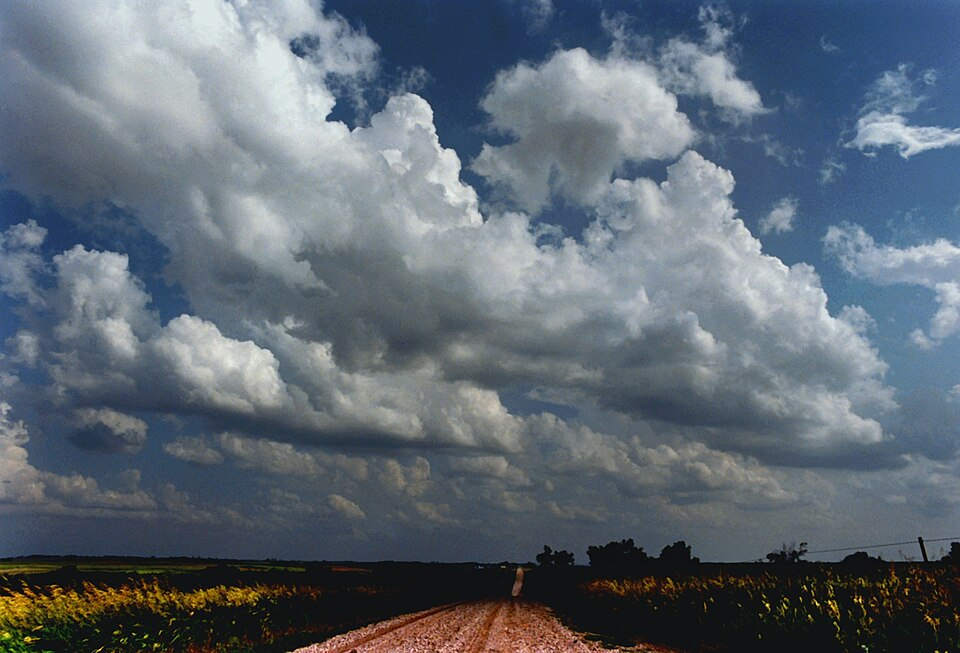
\includegraphics[width=\linewidth]{images/book1/g4-cumulus.jpg}

{\small \omterm{def:g4:clouds-rain-snow:cloud-families}{Cumulus}, heaped \omterm{def:g4:clouds-rain-snow:cloud}{clouds} with flat bases.}
\end{minipage}\hfill
\begin{minipage}[b]{0.49\linewidth}\centering
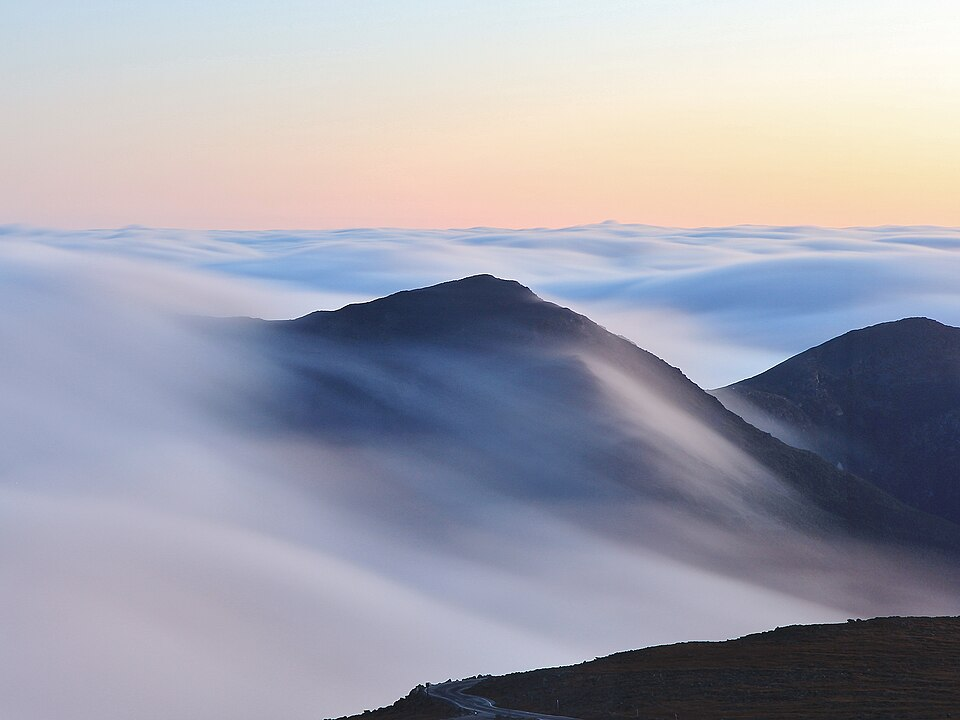
\includegraphics[width=\linewidth]{images/book1/g4-stratus.jpg}

{\small \omterm{def:g4:clouds-rain-snow:cloud-families}{Stratus}: a flat layer, here seen from above, from a \omterm{def:g1:landscapes-around-us:landform}{mountain}.}
\end{minipage}

\medskip
\begin{minipage}[b]{0.49\linewidth}\centering
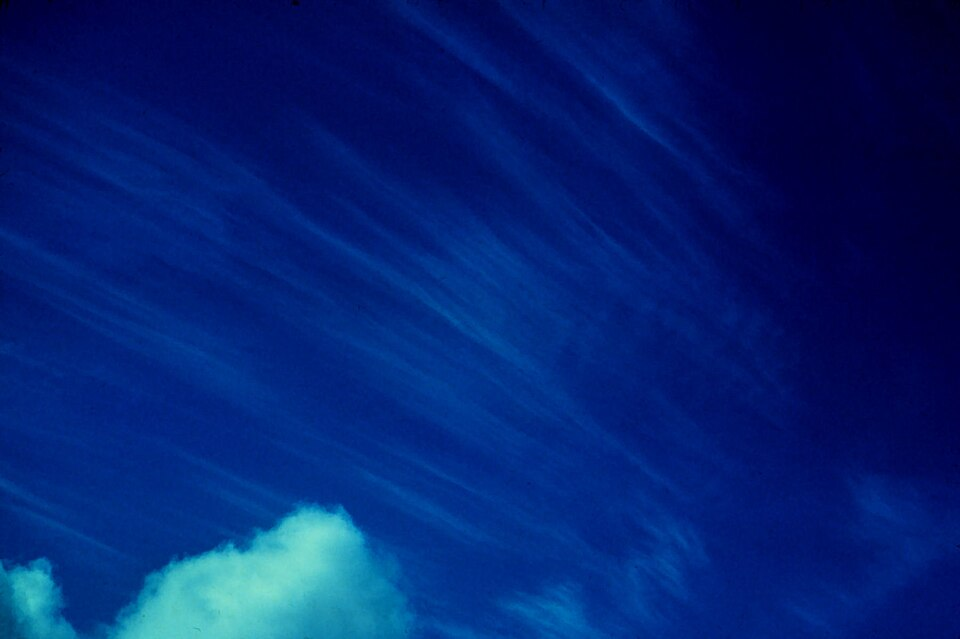
\includegraphics[width=\linewidth]{images/book1/g4-cirrus.jpg}

{\small \omterm{def:g4:clouds-rain-snow:cloud-families}{Cirrus}: thin threads of ice, very high (a small \omterm{def:g4:clouds-rain-snow:cloud-families}{cumulus} below).}
\end{minipage}\hfill
\begin{minipage}[b]{0.49\linewidth}\centering
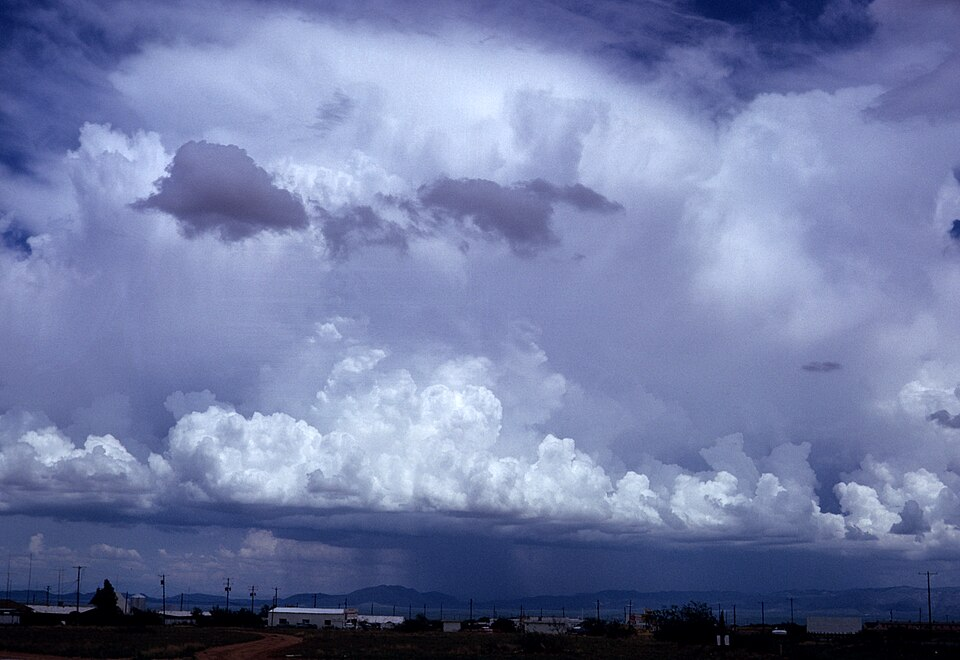
\includegraphics[width=\linewidth]{images/book1/g4-cumulonimbus.jpg}

{\small A \omterm{def:g4:clouds-rain-snow:cloud-families}{cumulonimbus}: a tower of \omterm{def:g4:clouds-rain-snow:cloud}{cloud}; \omterm{def:g4:clouds-rain-snow:precipitation}{rain} falls from its dark base.}
\end{minipage}

\smallskip
{\small Photographs: NOAA Photo Library (public domain): S. Corfidi
(\omterm{def:g4:clouds-rain-snow:cloud-families}{cumulus}), R. F. Kresge (\omterm{def:g4:clouds-rain-snow:cloud-families}{cirrus}), B. Hooke collection (\omterm{def:g4:clouds-rain-snow:cloud-families}{cumulonimbus}).}
% ledger: noaa:photos-g4
\label{fig:g4:clouds-rain-snow:photos}
\end{omfigure}

How high do \omterm{def:g4:clouds-rain-snow:cloud}{clouds} float? It depends on the family. Low \omterm{def:g4:clouds-rain-snow:cloud}{clouds}, like
\omterm{def:g4:clouds-rain-snow:cloud-families}{stratus} and the base of \omterm{def:g4:clouds-rain-snow:cloud-families}{cumulus}, float from just above the ground up to
about 2 kilometres. \omterm{def:g4:clouds-rain-snow:cloud-families}{Cirrus} float very high, between about 5 and 13
kilometres outside the tropics and the polar regions --- often higher than the highest
\omterm{def:g1:landscapes-around-us:landform}{mountain} on Earth.
A \omterm{def:g4:clouds-rain-snow:cloud-families}{cumulonimbus} stretches all the way from a low base to the very top of the
\omterm{def:g4:clouds-rain-snow:cloud}{cloud} levels.
% ledger: wmo:cloud-levels, wmo:cumulonimbus

\begin{omfigure}
\begin{tikzpicture}[x=1cm, y=0.5cm, font=\small]
  % height scale
  \draw[black!60] (0,0) -- (0,14);
  \foreach \h in {0,2,...,14} {
    \draw[black!60] (-0.1,\h) -- (0,\h);
    \node[anchor=east, font=\scriptsize] at (-0.12,\h) {\h\,km};
  }
  \node[anchor=south, font=\scriptsize, align=center] at (0,14.2) {height};
  % ground and a mountain for comparison
  \fill[green!35!black!50] (0.2,0) -- (11.4,0) -- (11.4,-0.4) -- (0.2,-0.4) -- cycle;
  \fill[black!35] (8.6,0) -- (9.9,8.8) -- (10.2,8.4) -- (11.2,0) -- cycle;
  \fill[white, draw=black!45, line width=0.3pt] (9.65,7.2) -- (9.9,8.8) -- (10.2,8.4) -- (10.4,7.0) -- (10.1,7.4) -- (9.9,7.0) -- cycle;
  \node[font=\scriptsize, align=center] at (9.9,10.2) {the highest\\mountain};
  % levels
  \fill[blue!6] (0.2,0.15) rectangle (8.3,2);
  \fill[blue!10] (0.2,5) rectangle (8.3,13);
  \node[anchor=west, font=\scriptsize, text=blue!50!black] at (0.3,1.65) {low clouds};
  \node[anchor=west, font=\scriptsize, text=blue!50!black] at (0.3,12.6) {high clouds};
  % stratus: a flat grey layer
  \fill[black!25, rounded corners=2pt] (0.6,0.6) rectangle (2.6,1.3);
  \node[font=\scriptsize] at (1.6,-1.1) {stratus};
  % cumulus
  \pic[scale=0.7, transform shape] at (4.0,0.9) {puffycloud};
  \node[font=\scriptsize] at (4.0,-1.1) {cumulus};
  % cirrus: wisps
  \foreach \y in {9.4,10.0,10.6} {
    \draw[black!50, line width=0.6pt] (0.8,\y) .. controls (1.4,\y+0.5) and (2.0,\y+0.1) .. (2.6,\y+0.6);
  }
  \node[font=\scriptsize] at (1.7,8.5) {cirrus};
  % cumulonimbus: tower with an anvil
  \fill[black!15, draw=black!45, line width=0.4pt]
    (5.4,1.0) .. controls (5.2,4) and (5.6,8) .. (5.9,11.2)
    .. controls (5.0,11.6) and (4.6,12.0) .. (4.8,12.3)
    -- (8.1,12.3) .. controls (8.2,12.0) and (7.8,11.6) .. (7.0,11.2)
    .. controls (7.3,8) and (7.6,4) .. (7.4,1.0) -- cycle;
  \fill[black!45] (5.4,1.0) rectangle (7.4,1.4);
  \foreach \x in {5.7,6.1,6.5,6.9,7.2}
    \draw[omWxRain, line width=0.6pt] (\x,0.95) -- (\x-0.15,0.15);
  \node[font=\scriptsize] at (6.4,-1.1) {cumulonimbus};
\end{tikzpicture}

{\small How high the four \omterm{def:g4:clouds-rain-snow:cloud}{cloud} families float (heights in kilometres, for
regions that are neither tropical nor polar). The \omterm{def:g4:clouds-rain-snow:cloud-families}{stratus} and the base of
the \omterm{def:g4:clouds-rain-snow:cloud-families}{cumulus} are low; \omterm{def:g4:clouds-rain-snow:cloud-families}{cirrus} are often higher than the highest \omterm{def:g1:landscapes-around-us:landform}{mountain}. A
\omterm{def:g4:clouds-rain-snow:cloud-families}{cumulonimbus} stretches from a low base to the top of the \omterm{def:g4:clouds-rain-snow:cloud}{cloud} levels.
Heights after the World Meteorological Organization's \omterm{def:g4:clouds-rain-snow:cloud}{cloud} atlas.}
\label{fig:g4:clouds-rain-snow:heights}
% ledger: wmo:cloud-levels, tht:everest
\end{omfigure}

\begin{method}[Naming a cloud]\label{met:g4:clouds-rain-snow:naming}
Look at the sky and ask three questions:
\begin{enumerate}
  \item Is it a heap with a flat base? Then it is a \omterm{def:g4:clouds-rain-snow:cloud-families}{cumulus} --- and if it
        rises into a huge dark tower, a \omterm{def:g4:clouds-rain-snow:cloud-families}{cumulonimbus}.
  \item Is it a flat, even sheet that hides the whole sky? Then it is a
        \omterm{def:g4:clouds-rain-snow:cloud-families}{stratus}.
  \item Is it made of thin white threads, very high? Then it is a \omterm{def:g4:clouds-rain-snow:cloud-families}{cirrus}.
\end{enumerate}
\end{method}

\begin{remark}[Clouds tell the weather]\label{rem:g4:clouds-rain-snow:tell}
Small \omterm{def:g4:clouds-rain-snow:cloud-families}{cumulus} in a blue sky mean fair \omterm{def:g1:watching-the-weather:weather}{weather}. A grey \omterm{def:g4:clouds-rain-snow:cloud-families}{stratus} brings a dull
day, sometimes with drizzle. A \omterm{def:g4:clouds-rain-snow:cloud-families}{cumulonimbus} brings a short, heavy shower,
often with thunder, lightning and gusts of wind --- sometimes \omterm{def:g4:clouds-rain-snow:precipitation}{hail}. \omterm{def:g4:clouds-rain-snow:cloud-families}{Cirrus}
bring no \omterm{def:g4:clouds-rain-snow:precipitation}{rain}, but when they spread and thicken, \omterm{def:g4:clouds-rain-snow:precipitation}{rain} often follows a day
later.
\end{remark}

\section{Rain, snow and hail}

Inside a \omterm{def:g4:clouds-rain-snow:cloud}{cloud}, the tiny droplets bump into one another and join, or ice
crystals grow at the expense of the droplets. A \omterm{def:g4:clouds-rain-snow:cloud}{cloud} drop, or a crystal,
that has grown big and heavy enough can no longer float: it falls.

\begin{definition}[Precipitation]\label{def:g4:clouds-rain-snow:precipitation}
\emph{Precipitation}\index{precipitation} is water that falls from a \omterm{def:g4:clouds-rain-snow:cloud}{cloud}
to the ground: \emph{rain}\index{rain} (drops of liquid water),
\emph{snow}\index{snow} (flakes made of ice crystals stuck together) or
\emph{hail}\index{hail} (balls of ice, called hailstones, that fall from
storm \omterm{def:g4:clouds-rain-snow:cloud}{clouds}).
\end{definition}

Whether it \omterm{def:g4:clouds-rain-snow:precipitation}{rains} or \omterm{def:g4:clouds-rain-snow:precipitation}{snows} depends on the temperature of the air the
\omterm{def:g4:clouds-rain-snow:precipitation}{precipitation} falls through. Snowflakes form high in the cold \omterm{def:g4:clouds-rain-snow:cloud}{cloud}. If
the air below is above \SI{0}{\celsius} for long enough, they melt on the
way down and reach us as \omterm{def:g4:clouds-rain-snow:precipitation}{rain}. If the air is freezing all the way to the
ground, they arrive as \omterm{def:g4:clouds-rain-snow:precipitation}{snow}.

\begin{omfigure}

\includegraphics[width=0.55\linewidth]{images/book1/ai/g4-snowflakes.jpg}

{\small Children catching snowflakes on a dark glove: each flake is made of
ice crystals.}
\end{omfigure}

\omterm{def:g4:clouds-rain-snow:precipitation}{Hail} falls only from \omterm{def:g4:clouds-rain-snow:cloud-families}{cumulonimbus}. Inside the tower, strong upward winds
carry ice pellets up and down several times; each trip adds a new layer of
ice, like the layers of an onion, until the hailstone is too heavy for the
wind to hold.

\begin{omfigure}
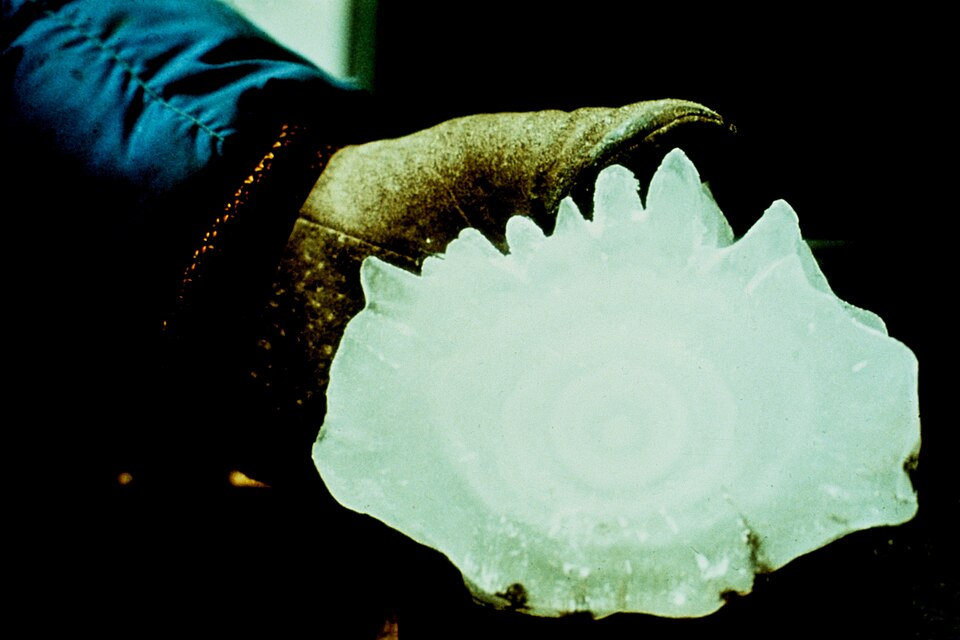
\includegraphics[width=0.5\linewidth]{images/book1/g4-hailstone.jpg}

{\small A very large hailstone held in a gloved hand. The rings show the
layers of ice it gathered inside the storm \omterm{def:g4:clouds-rain-snow:cloud}{cloud}. Photograph: NOAA Photo
Library (public domain).}
% ledger: noaa:photos-g4
\end{omfigure}

\section{Measuring the weather}

To say how much it rained, how warm it was or where the wind blew from,
words are not enough: we need instruments, and numbers.

\begin{definition}[Rain gauge]\label{def:g4:clouds-rain-snow:rain-gauge}
A \emph{rain gauge}\index{rain gauge} is a container that collects the \omterm{def:g4:clouds-rain-snow:precipitation}{rain}
falling on its opening. The depth of water it collects is measured in
millimetres: ``5 millimetres of \omterm{def:g4:clouds-rain-snow:precipitation}{rain}'' means that the \omterm{def:g4:clouds-rain-snow:precipitation}{rain} would have made
a layer of water 5 millimetres deep on flat ground, if none of it had run
off or soaked in.
\end{definition}

\begin{remark}[A millimetre of rain is a lot of water]\label{rem:g4:clouds-rain-snow:litre}
A millimetre of \omterm{def:g4:clouds-rain-snow:precipitation}{rain} looks tiny in the gauge. But on a square of ground one
metre by one metre, it is one litre of water: a big bottle. On a school
playground of one thousand square metres, a \omterm{def:g4:clouds-rain-snow:precipitation}{rain} of 10 millimetres brings
ten thousand litres: enough to fill a thousand buckets of 10 litres each.
\end{remark}

\begin{omfigure}
\begin{tikzpicture}[font=\small]
  % funnel
  \draw[black!70, line width=0.8pt] (-1.2,6.6) -- (-0.35,5.8) -- (-0.35,5.4);
  \draw[black!70, line width=0.8pt] (1.2,6.6) -- (0.35,5.8) -- (0.35,5.4);
  \draw[black!70, line width=0.8pt] (-1.2,6.6) -- (1.2,6.6);
  % tube
  \fill[blue!25] (-0.45,0) rectangle (0.45,2.4);
  \draw[black!70, line width=0.8pt] (-0.45,5.4) -- (-0.45,0) -- (0.45,0) -- (0.45,5.4);
  \foreach \m in {0,1,...,50} {
    \pgfmathsetmacro{\yy}{\m*0.1}
    \draw[black!60] (0.45,\yy) -- ++(-0.12,0);
  }
  \foreach \m in {0,5,10,...,50} {
    \pgfmathsetmacro{\yy}{\m*0.1}
    \draw[black!80] (0.45,\yy) -- ++(-0.25,0);
    \node[anchor=west, font=\scriptsize] at (0.5,\yy) {\m};
  }
  \node[anchor=west, font=\scriptsize] at (1.0,5.0) {mm};
  % reading line
  \draw[red!70!black, -{Stealth}] (-1.6,2.4) -- (-0.5,2.4);
  \node[anchor=east, align=right, font=\scriptsize] at (-1.65,2.4) {read the\\level here};
  \node[anchor=west, font=\scriptsize] at (1.9,2.4) {$\leftarrow$ 24\,mm of rain};
\end{tikzpicture}

{\small A simple \omterm{def:g4:clouds-rain-snow:rain-gauge}{rain gauge}: a funnel catches the \omterm{def:g4:clouds-rain-snow:precipitation}{rain} and a tube marked in
millimetres holds it. Read the level of the water, with your eye at the
same height. Here, 24 millimetres have fallen since the gauge was last
emptied.}
\label{fig:g4:clouds-rain-snow:gauge}
\end{omfigure}


\begin{definition}[Wind vane]\label{def:g4:clouds-rain-snow:wind-vane}
A \emph{wind vane}\index{wind vane} is an arrow that turns freely on a
mast. The wind pushes its tail, so the arrow always points to the
direction the wind is coming \emph{from}.
\end{definition}

\begin{definition}[Weather station]\label{def:g4:clouds-rain-snow:weather-station}
A \emph{weather station}\index{weather station} is a place where the \omterm{def:g1:watching-the-weather:weather}{weather}
is measured every day, always in the same way, with instruments: a
thermometer in a ventilated white box, a \omterm{def:g4:clouds-rain-snow:rain-gauge}{rain gauge} in the open, a \omterm{def:g4:clouds-rain-snow:wind-vane}{wind vane}
on a mast.
\end{definition}

The thermometer is kept in the shade, in a white box with slatted sides
that let the air through but keep out the sunshine and the \omterm{def:g4:clouds-rain-snow:precipitation}{rain}. The Met
Office, the \omterm{def:g1:watching-the-weather:weather}{weather} service of the United Kingdom, sets it
\SI{1.25}{\metre} above the ground. The \omterm{def:g4:clouds-rain-snow:rain-gauge}{rain gauge}
stands in the open, away from walls and trees that would shelter it from
the \omterm{def:g4:clouds-rain-snow:precipitation}{rain}, its opening a little above the ground. The \omterm{def:g4:clouds-rain-snow:wind-vane}{wind vane} stands high
on its mast, above the obstacles that would turn the wind.
% ledger: mo:screen-height, mo:raingauge

\begin{omfigure}
\begin{tikzpicture}[font=\small, x=1cm, y=1cm]
  % grass
  \fill[green!40!black!45] (-0.5,0) rectangle (11,-0.25);
  \foreach \x in {-0.3,0.1,...,10.8} \draw[green!45!black] (\x,0) -- ++(0.06,0.14);
  % screen on legs
  \draw[black!70, line width=1pt] (0.8,0) -- (0.8,1.25) (2.2,0) -- (2.2,1.25);
  \fill[white, draw=black!70] (0.6,1.25) rectangle (2.4,2.4);
  \foreach \y in {1.4,1.55,...,2.25} \draw[black!40] (0.7,\y) -- (2.3,\y-0.08);
  \fill[white, draw=black!70] (0.45,2.4) -- (1.5,2.75) -- (2.55,2.4) -- cycle;
  \draw[black!60, <->] (2.8,0) -- node[right, font=\scriptsize, align=left] {about\\1.25\,m} (2.8,1.25);
  \node[align=center, font=\scriptsize] at (1.5,3.25) {thermometer in a\\white slatted box};
  % rain gauge
  \fill[black!15, draw=black!70] (5.4,0) rectangle (5.9,0.4);
  \draw[black!70] (5.3,0.55) -- (5.4,0.4) (6.0,0.55) -- (5.9,0.4);
  \node[align=center, font=\scriptsize] at (5.65,1.2) {rain gauge,\\in the open};
  % tree far away
  \fill[brown!60!black] (7.3,0) rectangle (7.5,1.3);
  \fill[green!50!black!70] (7.4,2.1) circle (0.85);
  % wind vane on a mast
  \draw[black!70, line width=1pt] (9.8,0) -- (9.8,4.2);
  \draw[black!80, line width=1.4pt, -{Latex[length=3mm]}] (10.6,4.4) -- (9.0,4.4);
  \fill[black!80] (10.6,4.4) -- (10.9,4.65) -- (10.9,4.15) -- cycle;
  \node[align=center, font=\scriptsize] at (9.8,5.05) {wind vane on a high mast};
  \node[anchor=west, font=\scriptsize, align=left] at (10.1,3.4) {points to where\\the wind comes from};
\end{tikzpicture}

{\small A small \omterm{def:g4:clouds-rain-snow:weather-station}{weather station}. The thermometer is in the shade, in a white
box with slatted sides, about 1.25 metres above the grass; the \omterm{def:g4:clouds-rain-snow:rain-gauge}{rain gauge}
stands in the open, far from the tree; the \omterm{def:g4:clouds-rain-snow:wind-vane}{wind vane} is high above the
obstacles.}
\label{fig:g4:clouds-rain-snow:station}
% ledger: mo:screen-height
\end{omfigure}

\begin{inthefield}[A weather station in the schoolyard]
Many schools keep a small \omterm{def:g4:clouds-rain-snow:weather-station}{weather station} in a corner of the playground.
Every morning at the same time, two pupils read the thermometer, read and
empty the \omterm{def:g4:clouds-rain-snow:rain-gauge}{rain gauge}, and note where the \omterm{def:g4:clouds-rain-snow:wind-vane}{wind vane} points. Over the weeks,
the class builds a record of its own \omterm{def:g1:watching-the-weather:weather}{weather}.
\end{inthefield}

\begin{omfigure}
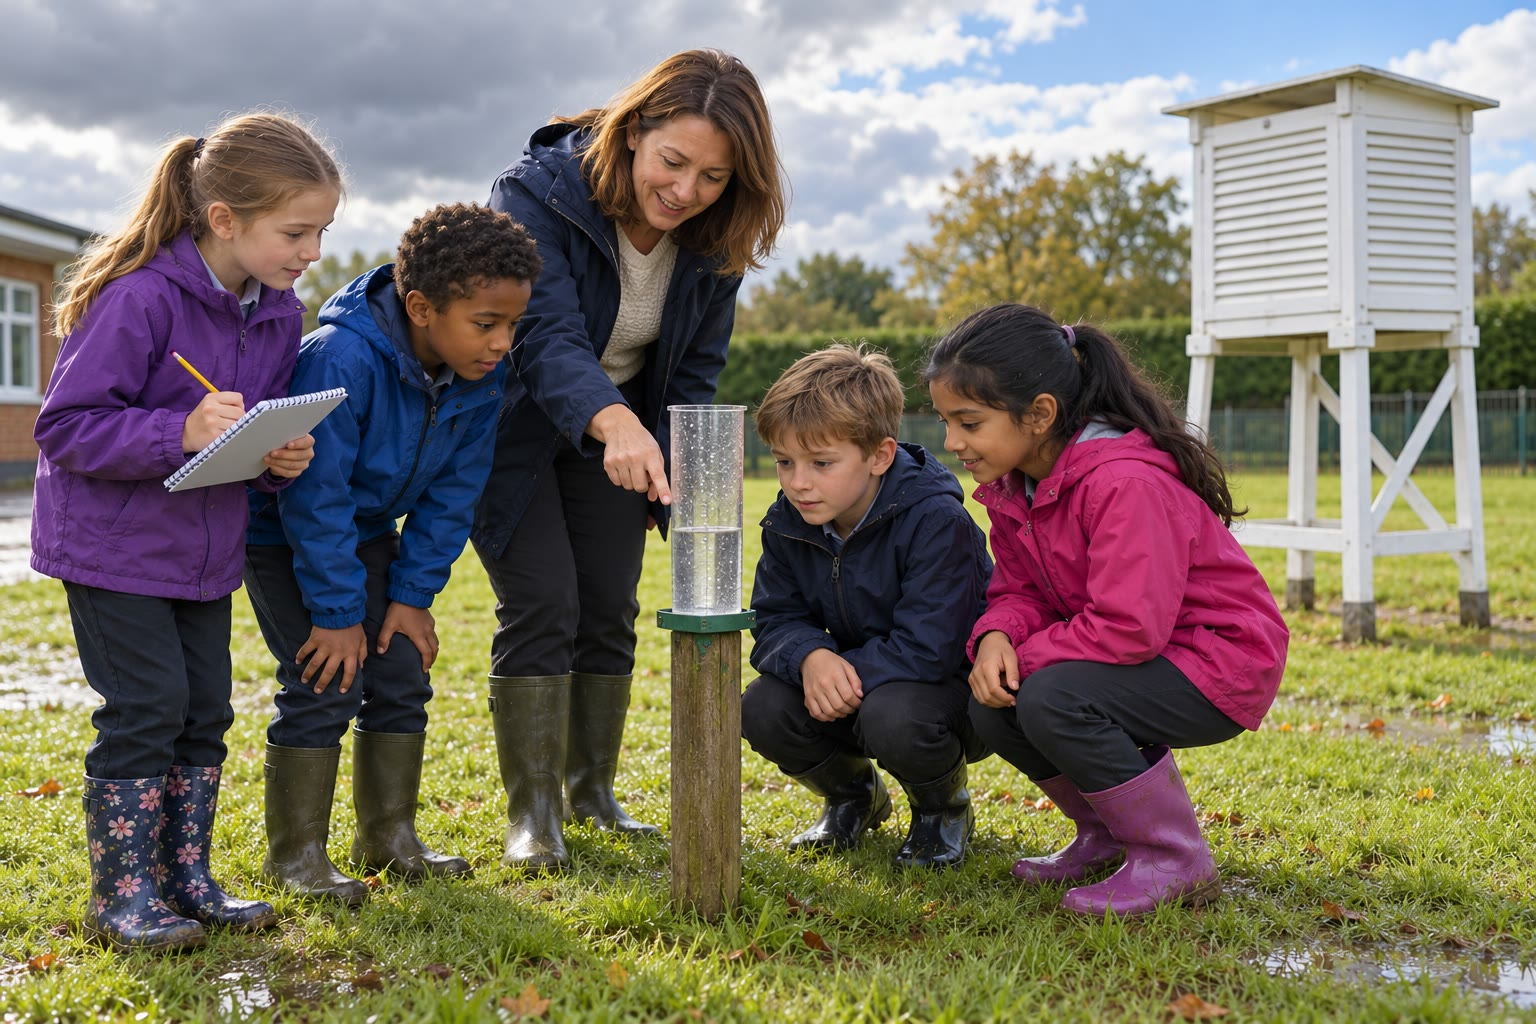
\includegraphics[width=0.55\linewidth]{images/book1/ai/g4-rain-gauge-class.jpg}

{\small Pupils reading the \omterm{def:g4:clouds-rain-snow:rain-gauge}{rain gauge} in the schoolyard.}
\end{omfigure}

\begin{method}[Drawing a bar chart of the rain]\label{met:g4:clouds-rain-snow:bar-chart}
To draw the \omterm{def:g4:clouds-rain-snow:precipitation}{rain} of a week:
\begin{enumerate}
  \item draw a horizontal line and write the days under it, equally spaced;
  \item draw a vertical line on the left and mark it in millimetres, with
        equal steps (for example every 2 millimetres);
  \item above each day, draw a bar as high as the \omterm{def:g4:clouds-rain-snow:precipitation}{rain} of that day; a day
        with no \omterm{def:g4:clouds-rain-snow:precipitation}{rain} gets no bar at all;
  \item give the chart a title and write the unit, mm, on the vertical
        line.
\end{enumerate}
\end{method}

\begin{example}[A week of rain at school]\label{ex:g4:clouds-rain-snow:week}
The class read the \omterm{def:g4:clouds-rain-snow:rain-gauge}{rain gauge} every morning for a week and found: Monday 0,
Tuesday 4, Wednesday 12, Thursday 7, Friday 0, Saturday 2, Sunday 5
millimetres. The wettest day was Wednesday. It did not \omterm{def:g4:clouds-rain-snow:precipitation}{rain} on Monday nor on
Friday. In the whole week, $0 + 4 + 12 + 7 + 0 + 2 + 5 = 30$ millimetres
fell. Wednesday alone brought 12 of the 30 millimetres, that is
$\frac{12}{30} = \frac{2}{5}$ of the week's \omterm{def:g4:clouds-rain-snow:precipitation}{rain}.
\end{example}

\begin{omfigure}
\begin{tikzpicture}
\begin{axis}[ybar, bar width=14pt, width=0.8\linewidth, height=5.4cm,
    ymin=0, ymax=14, ytick={0,2,...,14}, ylabel={rain (mm)},
    symbolic x coords={Mon,Tue,Wed,Thu,Fri,Sat,Sun}, xtick=data,
    axis x line*=bottom, axis y line*=left, ymajorgrids, grid style={gray!25},
    nodes near coords, nodes near coords style={font=\scriptsize},
    every axis label/.append style={font=\small}, tick label style={font=\small},
    title={Rain at school, one week}, title style={font=\small}]
  \addplot[fill=omWxRain!70, draw=omWxRain!60!black] coordinates
    {(Mon,0) (Tue,4) (Wed,12) (Thu,7) (Fri,0) (Sat,2) (Sun,5)};
\end{axis}
\end{tikzpicture}

{\small The week of \cref{ex:g4:clouds-rain-snow:week} as a bar chart.}
\label{fig:g4:clouds-rain-snow:bars}
\end{omfigure}

\section{Exercises}

\begin{exercise}[$\star$]\label{exo:g4:clouds-rain-snow:1}
What is a \omterm{def:g4:clouds-rain-snow:cloud}{cloud} made of? What is \omterm{def:g4:clouds-rain-snow:cloud}{fog}?
\end{exercise}

\begin{exercise}[$\star$]\label{exo:g4:clouds-rain-snow:2}
Name the \omterm{def:g4:clouds-rain-snow:cloud}{cloud}: (a) a flat grey sheet that hides the whole sky; (b) thin
white threads very high in a blue sky; (c) white heaps with flat bases, like
cotton wool; (d) a huge dark tower with a flat top, bringing thunder.
\end{exercise}

\begin{exercise}[$\star$]\label{exo:g4:clouds-rain-snow:3}
\omterm{def:g4:clouds-rain-snow:precipitation}{Rain}, \omterm{def:g4:clouds-rain-snow:precipitation}{snow} or \omterm{def:g4:clouds-rain-snow:precipitation}{hail}? (a) balls of ice that fall from a storm \omterm{def:g4:clouds-rain-snow:cloud}{cloud}; (b) drops
of liquid water; (c) flakes made of ice crystals.
\end{exercise}

\begin{exercise}[$\star$]\label{exo:g4:clouds-rain-snow:4}
Which instrument measures: (a) the \omterm{def:g4:clouds-rain-snow:precipitation}{rain}; (b) the temperature; (c) where the
wind comes from?
\end{exercise}

\begin{exercise}[$\star$]\label{exo:g4:clouds-rain-snow:5}
In the \omterm{def:g4:clouds-rain-snow:rain-gauge}{rain gauge} drawn on page~\pageref{fig:g4:clouds-rain-snow:gauge}, the water now
reaches the mark 17. How many millimetres of \omterm{def:g4:clouds-rain-snow:precipitation}{rain} have fallen? How many
more millimetres would bring it to 20?
\end{exercise}

\begin{exercise}[$\star$]\label{exo:g4:clouds-rain-snow:6}
Look at the bar chart on page~\pageref{fig:g4:clouds-rain-snow:bars}. Which day
was the wettest? On which days did it not \omterm{def:g4:clouds-rain-snow:precipitation}{rain}? Which day had 7
millimetres?
\end{exercise}

\begin{exercise}[$\star\star$]\label{exo:g4:clouds-rain-snow:7}
On the morning of a snowy day, the snowflakes reach the ground in the
\omterm{def:g1:landscapes-around-us:landform}{mountain} village, but in the \omterm{def:g1:landscapes-around-us:landform}{valley} below it \omterm{def:g4:clouds-rain-snow:precipitation}{rains}. Explain the difference,
using the temperature of the air.
\end{exercise}

\begin{exercise}[$\star\star$]\label{exo:g4:clouds-rain-snow:8}
Another week, the class finds: Monday 3, Tuesday 0, Wednesday 1, Thursday
9, Friday 6, Saturday 0, Sunday 1 millimetres. Draw the bar chart. How many
millimetres fell in the week? Which fraction of the week's \omterm{def:g4:clouds-rain-snow:precipitation}{rain} fell on
Thursday?
\end{exercise}

\begin{exercise}[$\star\star$]\label{exo:g4:clouds-rain-snow:9}
Why must the \omterm{def:g4:clouds-rain-snow:rain-gauge}{rain gauge} stand in the open, far from walls and trees? Why
is the thermometer kept in a white box in the shade, and not in full sun?
\end{exercise}

\begin{exercise}[$\star\star$]\label{exo:g4:clouds-rain-snow:10}
The \omterm{def:g4:clouds-rain-snow:wind-vane}{wind vane} points to the west. Where does the wind come from? Where is
it going?
\end{exercise}

\begin{exercise}[$\star\star\star$]\label{exo:g4:clouds-rain-snow:11}
On a playground of 500 square metres, 8 millimetres of \omterm{def:g4:clouds-rain-snow:precipitation}{rain} fall. Using
\cref{rem:g4:clouds-rain-snow:litre}, how many litres of water fell on the
playground? A watering can holds 10 litres: how many watering cans is that?
\end{exercise}
